\section{Theorie}
\label{sec:Theorie}

\subsection{Die paramagnetische Suszeptibilität}
\label{subsec:theoriesuszeptibilitaet}
Bei Anwesenheit von Materie hängen magnetische Flussdichte $\symbf{B}$, externe
magnetische Feldstärke $\symbf{H}$, magnetische Permeabilität des Vakuums $\mu_0$
und Magnetisierung des Materials $\symbf{M}$ durch
\begin{equation}
  \symbf{B} = \mu_0 \symbf{H} + \symbf{M}
  \label{eqn:bhm}
\end{equation}
zusammen. Die Magnetisierung $\symbf{M}$ beschreibt hierbei die Dichte der
magnetischen Dipolmomente im Material und hängt durch
\begin{equation}
  \symbf{M} = \mu_0 \chi \symbf{H}
  \label{eqn:mchih}
\end{equation}
von dem externen Magnetfeld $\symbf{H}$ ab. Dabei ist die Proportionalitätskonstante
$\chi$ die magnetische Suszeptibilität. Im einfachsten Fall ist sie eine materialabhängige
Konstante, kann aber im allgemeinen Fall vom externen Magnetfeld und der Temperatur $T$
des Materials abhängen.
In diesem Versuch wird die Suszeptibilität paramagnetischer Substanzen untersucht.
Nur Atome, Moleküle oder Ionen mit nicht verschwindendem Drehimpuls weisen
Paramagnetismus auf. Dieser beruht darauf, dass sich magnetische Momente parallel zu
einem äußeren Magnetfeld ausrichten. Da thermische Bewegungen dies stören, ist der Effekt
temperaturabhängig. Da der atomare Drehimpuls mit dem magnetischen Moment gekoppelt ist,
soll dieser Zusammenhang erläutert werden. \\
Der Gesamtdrehimpuls $\symbf{J}$ eines Atoms setzt sich aus dem Bahndrehimpuls
$\symbf{L}$ der Elektronenhülle, dem Eigendrehimpuls, dem sogenannten Spin, $\symbf{S}$
und dem Kernspin, der für paramagnetische Effekte vernachlässigt werden kann, zusammen.
Unter die Voraussetzung eines nicht zu starken Magnetfeldes addieren sich beide
Drehimpulse zu einem Gesamtdrehimpuls $\symbf{J}$ durch
\begin{equation}
  \symbf{J} = \symbf{L} + \symbf{S}\,.
  \label{eqn:ls}
\end{equation}
Es kann angenommen werden, dass sich $\symbf{L}$ und $\symbf{S}$ als ungewichtete vektorielle
Summe der einzelnen Bahndrehimpulse $\symbf{l}_{\text{i}}$ und Spins $\symbf{s}_{\text{i}}$ ergeben.
Die Addition zu einem Gesamtdrehimpuls wird als LS-Kopplung bezeichnet. Für die
resultierenden magnetischen Momente gilt dann
\begin{align}
  \symbf{\mu_{\text{L}}} &= - \frac{\mu_{\text{B}}}{\hbar} \symbf{L} \,\\
  \symbf{\mu_{\text{S}}} &= - g_{\text{S}} \frac{\mu_{\text{B}}}{\hbar} \symbf{S} \,.
  \label{eqn:mulmus}
\end{align}
Dabei bezeichnet $\mu_{\text{B}}$ das Bohrsche Magneton, $\hbar$ das reduzierte Plancksche
Wirkungsquantum und $g_{\text{S}}$ das gyromagnetische Verhältnis des freien Elektrons.
Allgemein gilt die Relation
\begin{equation}
  |\symbf{N}| = \sqrt{(N(N+1))} \hbar
\end{equation}
für einen der drei Drehimpulse als $\symbf{N}$ mit seiner dazugehörigen Quantenzahl
$N$. Damit ergeben sich die Beträge der magnetischen Momente zu
\begin{align}
  |\symbf{\mu_{\text{L}}}| &= \mu_{\text{B}} \sqrt{L(L+1)} \, \\
  |\symbf{\mu_{\text{S}}}| &= g_{\text{S}} \mu_{\text{B}} \sqrt{S(S+1)} \, .
\end{align}
Dabei ist $L$ die Bahndrehimpulsquantenzahl und $S$ die Spinquantenzahl.
Mit $\symbf{\mu}_{\text{J}}$ sei der zu $\symbf{J}$ parallele Anteil des zum Gesamtdrehimpuls $\symbf{J}$
gehörigen magnetischen Moments $\symbf{\mu}$ bezeichnet.

\begin{figure}
  \centering
  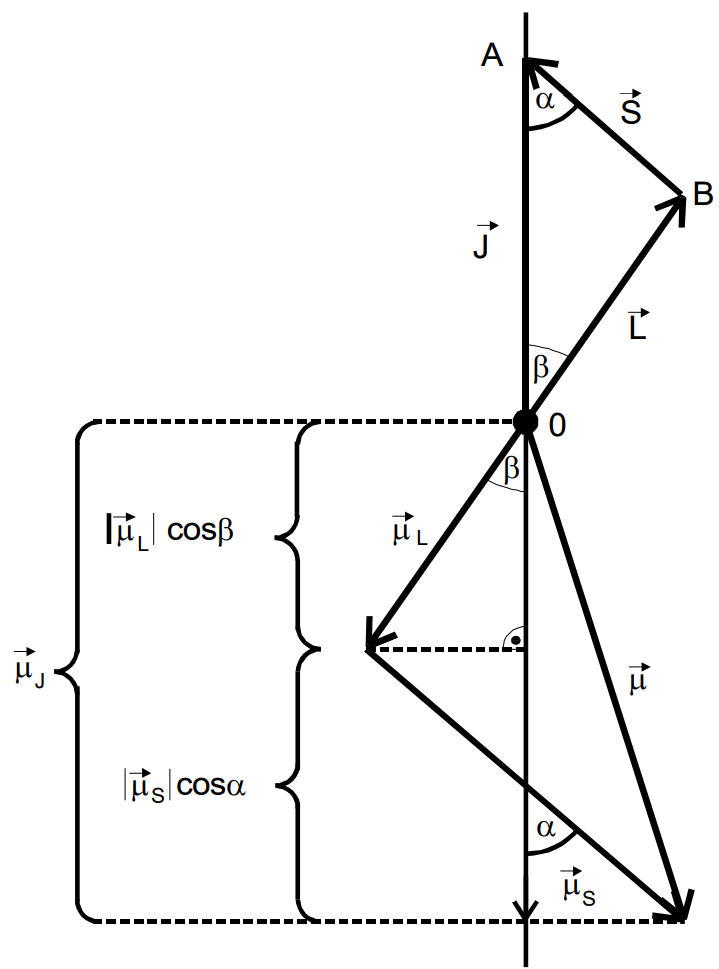
\includegraphics[width=180pt]{data/drehimpulse.png}
  \caption{Vektorielle Veranschaulichung zu den atomaren Drehimpulsen und den magnetischen Momenten \cite{Versuchsanleitung}.}
  \label{fig:vektordreh}
\end{figure}

Aus Abbildung \ref{fig:vektordreh} lässt sich die Beziehung
\begin{equation}
  |\symbf{\mu}_{\text{J}}| = |\symbf{\mu}_{\text{S}}| \cos\alpha + |\symbf{\mu}_{\text{L}}| \cos\beta\,.
  \label{eqn:cos}
\end{equation}
Mithilfe des Kosinussatzes und dem Einsetzen der oben ausgerechneten Beträge der magnetischen Momente in Gleichung
\ref{eqn:cos} folgt
\begin{equation}
  |\symbf{\mu}_{\text{J}}| \approx \mu_{\text{B}} g_{\text{J}} \sqrt{J(J+1)}\,,
\end{equation}
dabei wird der Ausdruck
\begin{equation}
  g_{\text{J}} = \frac{3J(J+1) + (S(S+1)-L(L+1))}{2J(J+1)}
  \label{eqn:lande}
\end{equation}
der Landé-Faktor des Atoms genannt und das gyromagnetische Verhältnis des Elektrons wurde
mit 2 angenähert. \\
Zwischen der Richtung des äußeren Magnetfeldes und der Richtung von $\symbf{\mu}_{\text{J}}$
sind nicht beliebige Winkel möglich. Dies wird Richtungsquantelung genannt. Für die Komponente
$\mu_{\text{J}_{\text{z}}}$ von $\symbf{\mu}_{\text{J}}$ gilt dann
\begin{equation}
  \mu_{\text{J}_{\text{z}}} = - \mu_{\text{B}} g_{\text{J}} m\,.
\end{equation}
Dabei ist $m$ ganzzahlig und wird Orientierungs- oder magnetische Quantenzahl genannt.
Der Wertebereich von $m$ ist begrenzt, es gibt $2J+1$ Möglichekiten. Zu jedem $m$ gibt es also eine bestimmte Richtung
des magnetischen Moments mit einer bestimmten potentiellen Energie, woraus sich die
Magnetisierung $\symbf{M}$ einer makroskopischen Probe berechnen lässt.
Dazu wird über das Produkt der Auftrittswahrscheinlichkeit der bestimmten
Orientierung der magnetischen Momente mit ihren Beträgen summiert.
Schlussendlich ergibt sich in Näherung von Zimmertemperatur und Feldern in der Größenordnung
von bis zu einem Tesla für die Magnetisierung und die paramagnetische Suszeptibilität
\begin{align}
  &M = \frac{1}{3} \mu_0 \mu_{\text{B}}^2 g_{\text{J}}^2 N \frac{J(J+1)B}{k_\text{B}T} \,\\
  &\chi = \frac{\mu_0 \mu_{\text{B}}^2 g_{\text{J}}^2 N J (J+1)}{3 k_{\text{B}} T}\,.
  \label{eqn:theoriewert}
\end{align}
Dabei bezeichnet $k_\text{B}$ die Boltzmann-Konstante, $T$ ist die Temperatur.
Es ist ersichtlich, dass die Suszeptibilität invers in Hochtemperaturnäherung
zum Inversen der Temperatur ist. Dies ist auch als Curiesches Gesetz des Paramagnetismus bekannt.

\subsection{Berechnung der quantenmechanischen Größen für Verbindungen von Metallen der seltenen Erden}
\label{subsec:berechnungquantenzahlenundlande}
Ionische Verbindungen der Metalle seltener Erden zeigen starken Paramagnetismus.
Um diesen zu untersuchen, ist es zuvor nötig, die Quantenzahlen $S$, $L$ und $J$ sowie
den Landé-Faktor der Verbindung zu berechnen. Die Hundschen Regeln treffen Aussagen
über die konkrete Konfiguration der Elektronen in den Orbitalen im Grundzustand.
Eine Formulierung dieser Regeln lautet:

1. Unter allen Konfigurationen, die das Pauli-Prinzip noch erlaubt, wird zunächst die
angenommen, bei der der Gesamtspin $\symbf{S} = \sum \symbf{s}_{\text{i}}$ maximal ist.

2. Unter allen Konfigurationen, die das Pauli-Prinzip und die erste Regel erlauben, wird
die angenommen, bei der der Gesamtbahndrehimpuls $\symbf{L} = \sum \symbf{l}_{\text{i}}$
maximal ist.

3. Der Gesamtdrehimpuls $\symbf{J}$ beträgt für weniger als halb gefüllte Schalen
$\symbf{J} = \symbf{L} - \symbf{S}$ und für mehr als halb gefüllte Schalen
$\symbf{J} = \symbf{L} + \symbf{S}$.

Es sei angemerkt, dass für genau halb volle Schalen beide Formeln in Regel 3 das gleiche
Ergebnis liefern, sodass auch dieser Fall durch Anwendung einer der beiden Formeln
gedeckt ist.
In diesem Versuch werden die Verbindungen $\ce{Dy2O3}$, $\ce{C6O12Pr2}$, $\ce{Gd2O3}$ und $\ce{Nd2O3}$ verwendet, sodass die dreifach positiv geladenen
Ionen $\ce{Dy^{3+}}$, $\ce{Pr^{3+}}$, $\ce{Gd^{3+}}$, $\ce{Nd^{3+}}$ betrachtet werden.
Die sich ergebenden Quantenzahlen und Landé-Faktoren sind in Tabelle \ref{tab:lsjg}
dargestellt. Die Größen ergeben sich durch konsistente Anwendung der Hundschen Regeln
auf die angegebene Elektronenkonfiguration, wobei beachtet wird, dass volle Schalen nicht beitragen.
Der Landé-Faktor wird mit Gleichung \eqref{eqn:lande} berechnet.

\begin{table}[H]
\begin{center}
\caption{Gemäß den Hundschen Regeln bestimmte Werte für die relevanten Quantenzahlen und den Landé-Faktor der Ionen.}
\label{tab:lsjg}
\begin{tabular}{cccccc}
\toprule
Ion & Elektronenkonfiguration & $L$ & $S$ & $J$ & $g_{\text{J}}$\\
\midrule
$\ce{Dy^{3+}}$ & $[\text{Xe}] \, 4f^9$ & $5$ & $5/2$ & $15/2$ & $4/3$  \\
$\ce{Pr^{3+}}$ & $[\text{Xe}] \, 4f^2$ & $5$ & $1$   & $4$    & $4/5$  \\
$\ce{Gd^{3+}}$ & $[\text{Xe}] \, 4f^7$ & $0$ & $7/2$ & $7/2$  & $2$    \\
$\ce{Nd^{3+}}$ & $[\text{Xe}] \, 4f^3$ & $6$ & $3/2$ & $9/2$  & $8/11$ \\
\bottomrule
\end{tabular}
\end{center}
\end{table}

\subsection{Apparatur zur Messung der Suszeptibilität}
\label{subsec:apparatur}

Die Suszeptibilität einer Probe lässt sich im Prinzip durch die Messung
der Induktivität einer Spule bestimmen. Hier werden zwei Spulen mit möglichst gleicher
Induktivität verwendet. Diese werden zu einer Brückenschaltung verbunden, die in Abbildung
\ref{fig:brueckenschaltung} zu sehen ist.

\begin{figure}
  \centering
  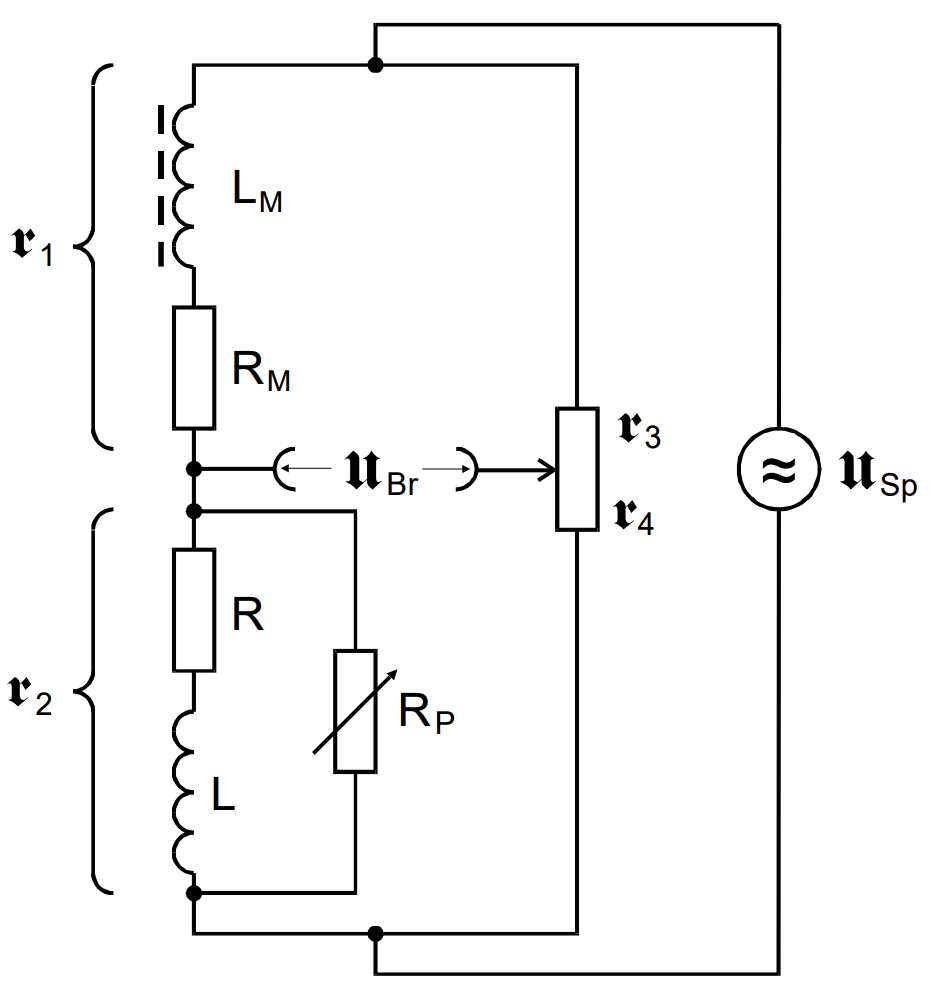
\includegraphics[width=180pt]{data/bruecke.png}
  \caption{Brückenschaltung zur Bestimmung der Suszeptibilität einer Probe\cite{Versuchsanleitung}.}
  \label{fig:brueckenschaltung}
\end{figure}

Die Brückenschaltung, aus der sich die Suszeptibilität bestimmen lässt, wird mit $U_\text{Br}$ bezeichnet.
Es lässt sich dann zeigen, dass für große Kreisfrequenzen $\omega$ mit der Bedingung
$(\omega^2 L ^2) \gg R^2$ bei zunächst abgeglichener Brücke
\begin{equation}
  \chi(\omega \to \infty) = 4 \frac{F}{Q} \frac{U_\text{Br}}{U_\text{Sp}}
  \label{eqn:spannung}
\end{equation}
gilt, wobei $U_\text{Br}$ die Brückenspannung nach Befüllung der Spule mit der Probe,
$F$ die Spulenquerschnittsfläche, $Q$ die Probenquerschnittsfläche und $U_\text{Sp}$ die Speisespannung bezeichnet.
Eine zweite Möglichkeit, die Suszeptibilität zu bestimmen, besteht darin, nach dem Befüllen
einer Spule die Brücke erneut abzugleichen. Dann ist die Brückenspannung abgesehen von Störspannungen
null und die Suszeptibilität kann mit dieser Methode zu
\begin{equation}
  \chi = 2 \frac{\Delta R}{R_3} \frac{F}{Q}
  \label{eqn:widerstand}
\end{equation}
berechnet werden. Dabei bezeichnet $R_3$ den Widerstand am Potentiometer und $\Delta R$
die Änderung des Widerstands, die nötig ist, um die Brückenspannung nach Befüllen
einer Spule mit der Probe wieder nahezu auf null zu bringen.

Es ist zu beachten, dass bei konkreter Berechnung $Q$ hier gleich $Q_\text{real} =  \frac{M_\text{p}}{L \rho_\text{w}}$
zu setzen ist. Dies beruht darauf, dass die Proben staubförmig sind und nicht beliebig
dicht gepackt werden können. Die Masse der Probe ist $M_\text{p}$ und die Dichte eines Einkristalls
des Probenmaterials wird mit $\rho_\text{w}$ bezeichnet.

Da die Brückenspannung durch Störspannung den Ausgangsklemmen der Brückenschaltung
überdeckt wird, wird die zu messende Spannung verstärkt und gefiltert. Dies ist deswegen möglich, weil
die zu messende Spannung monofrequent ist. Der verwendete sogenannte Selektivverstärker
ist in der Lage, Störspannungen größtenteils herauszufiltern und das Signal ausreichend zu verstärken.
Die Filterkurve des Selektivverstärkers ist eine Gauß-Kurve.
